\svnid{$Id: quickplot.tex 74563 2022-02-13 20:35:17Z jagers $}

\chapter{\DQUICKPLOT\ functionality} \label{Chp:QuickPlot}
The \DQUICKPLOT\ interface can be started by typing \command{d3d\_qp} at the MATLAB command prompt.
This interface is intended to simplify the creation of plots with MATLAB.
Tooltips provide online help for the interface.
The same interface is also available as a standalone program.
This chapter gives only a short introduction; for a detailed description of the interface, you are referred to the \DQUICKPLOT\ manual \citep{QP_UM}.

\begin{figure}
\center{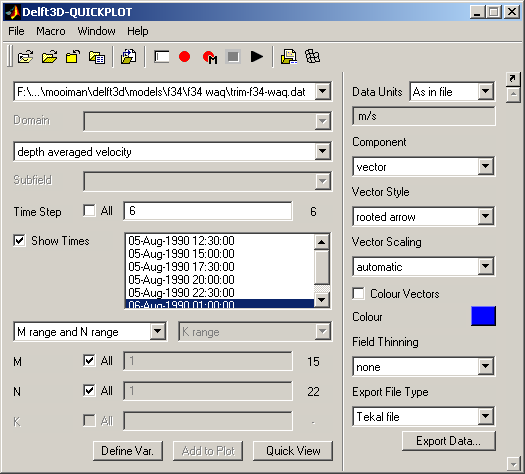
\includegraphics[width=125mm]{matlab/selection_window_qp.png}}
\caption{Selection window of \DQUICKPLOT.}
\label{fig:4.1}
\end{figure}

The interface allows to open NEFIS files and select data fields.
After making a selection of time steps, stations and m, n, k indices, you can either load the data (\button{Load Data} button) or plot the data (by clicking the \button{Quick View} or \button{Quick Animate} button).

The \button{Load Data} button in the lower left corner of the interface is not available in the standalone version, so it is described here.
When the data is loaded using the \button{Load Data} button, a workspace variable called 'data' is created.
If the variable 'data' was already defined any data contained in it will be overwritten without confirmation.
The variable 'data' contains:

\begin{itemize}
\item a field X with the x co-ordinates
\item a field Y with the y co-ordinates
\item a field Z with the z co-ordinates (for 3D data sets only)
\item a field Val with the data is the data is scalar
\item fields XComp, YComp and ZComp when the data is a vector quantity.
\end{itemize}

The same functionality can be accessed from the command line using the command

\begin{Verbatim}
X=d3d_qp('loaddata')
\end{Verbatim}

In this case the data is assigned to the user-specified variable X.
Many of the other functionalities of \DQUICKPLOT\ can also be accessed from the command line.
The general syntax of these commands is:

\begin{Verbatim}
d3d_qp(command_string,...command_parameters...)
\end{Verbatim}

The \command{command\_string} identifies the functionality that should be activated, e.g. 'loaddata', 'openfile' or 'colourbar'.
The \command{command\_parameters} depend on the command chosen, e.g. 'loaddata' does not need any parameter, 'openfile' does not need any parameter either but if a parameter is specified then it should be the name of the file to be opened, and 'colourbar' requires one parameter namely a 1 or 0 to indicate whether a colourbar should be drawn or not.
The details of all these commands is not described here.
The best way to learn these commands is by doing.
Therefore, \DQUICKPLOT\ has several options to display or export the equivalent commands that it is executing when you click on its buttons.
These display options can be accessed from the Macro menu of \DQUICKPLOT\ as shown in \Fref{fig:4.2}.

\begin{figure}
\center{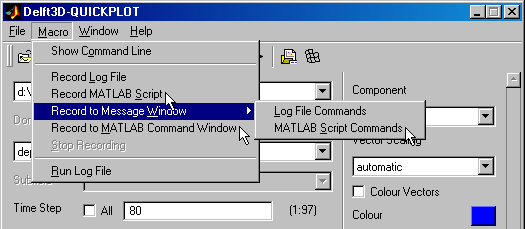
\includegraphics[width=100mm]{matlab/4-2.png}}
\caption{Display/export options for QUICKPLOT\ commands.}
\label{fig:4.2}
\end{figure}

For exporting/displaying the MATLAB commands associated with the various functionalities of \DQUICKPLOT, the following three options are available:

\begin{itemize}
\item Record MATLAB Script.
Records the commands directly to a MATLAB .m file.
\item Record to Message Window, MATLAB Script Commands.
Records the commands in a separate window of \DQUICKPLOT.
The commands cannot be copied from this window, but the recorded commands can be saved to a text file.
\item Record to MATLAB Command Window (not available in the standalone version of \DQUICKPLOT).
Echoes the commands to the MATLAB Command Window from which they can be easily copied.
When using MATLAB's diary option, the echoed commands will also end up in the diary file.
\end{itemize}

Both \DQUICKPLOT\ log files and MATLAB script files containing \DQUICKPLOT\ calls can be run using the Run Log File menu item of \DQUICKPLOT.
The MATLAB script files may also contain other single line MATLAB function calls (not supported in standalone mode).
Scripts containing multi-line MATLAB constructs cannot be run from within the \DQUICKPLOT\ interface.

When the data is plotted or animated a new figure is opened.
Scaling of axes, vector length and colours is automatic.
This implies that during an animation colour scaling, vector length scaling and plot extent may vary.
The plot extent and colour scaling can be set using the MATLAB commands \command{axis}, \command{set}, \command{gca} and \command{colorbar}.
For example:

\begin{Verbatim}
axis([xmin xmax ymin ymax]) % set the axes extent
\end{Verbatim}

and

\begin{Verbatim}
set(gca,'clim',[cmin cmax]) % set the colour limits
colorbar % update the colourbar
\end{Verbatim}

\begin{figure}
\center{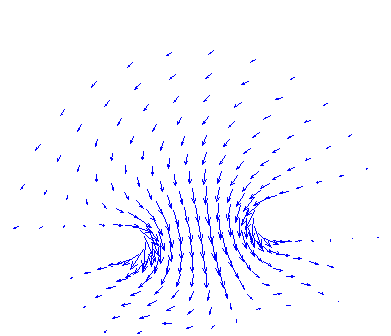
\includegraphics{matlab/standard_vector_plot.png}}
\caption{Example of \DQUICKPLOT\ figure.}
\label{fig:4.3}
\end{figure}

In case of an animation, plotting can be stopped by either closing the figure or selecting the Stop option from the Animation menu in the figure of the plot.
When the data set contains multiple time steps, a scroll bar will be plotted in the lower left corner of the plot figure.
You can use this to change the time step of the plot.

\begin{Remark}
\item The figure files saved by the standalone version of \DQUICKPLOT\ are compatible with MATLAB 6.5.
It does not support files created with newer MATLAB versions.
\item Access to netCDF files and data on OPeNDAP enabled websites requires the 'mexnc' and 'snctools' toolboxes available from \url{http://mexcdf.sourceforge.net/}.
The files of those toolboxes are now included in the netcdf subdirectory of the \DMATLAB distribution and should be automatically added to the search path when running \command{d3d\_qp} or \command{qpfopen}.
\end{Remark}
